\chapter[Theoretical Review][Theoretical Review]{Theoretical Review}
\label{chap:standardmodel}

The Standard Model of particle physics is the preeminent theory describing the behavior of subatomic particles. It has been rigorously tested for many decades and is the result of generations of experimental observations crossed with theoretical interpretations. Until recently, a fundamental particle of the theory had not been observed: the Higgs boson. The particle was first observed by the ATLAS and CMS experiments at the LHC in 2012.

\section{The Standard Model}

The Standard Model (SM) describes how particles in nature interact in the electroweak and quantum chromodynamic (QCD) sectors. These interactions are encoded in the SM Lagrangian written in the language of a quantum field theory, where particles are represented by quantum fields. The SM Lagrangian is a non-abelian gauge theory with the symmetry group $\text{SU(3)}\times\text{SU(2)}\times\text{U(1)}$. 

The gauge invariance of $\text{SU(3)}$, $\text{SU(2)}$, and $\text{U(1)}$ implies the existent of the eight gluon fields which mediate QCD, the three $W^\text{1,2,3}$ bosons which mediate the weak sector, and the $B$ boson which mediates the electromagnetic sector. All of these bosons are predicted to be massless, though, which presents a problem since the weak forces are known to be short range, i.e., their mediating boson ought to be massive.

This problem was remedied independently by Brout and Englert~\cite{1964.Englert.symmetry_breaking}, Higgs~\cite{1964.Higgs.Broken_Symmetries_1,1964.Higgs.Broken_Symmetries_2}, and Guralnik, Hagen, and Kibble~\cite{1964.Guralnik-Hagen-Kibble.symmetry_breaking} in the 1960s. They proposed the symmetry be spontaneously broken by a new scalar field whose accompanying particle has been dubbed the Higgs boson, and the result of this breaking are the massive $W^\pm$ and $Z$ fields, which are superpositions of the massless $W^\text{1,2,3}$ and $B$ bosons. 

Another observable aspect of this theory of electroweak symmetry breaking is the mixing angle $\theta_W$, which governs the mixing of the $B$ and the $W_\text{0}$ into the $Z$ and photon~\cite{}. A handful of experiments in the 1970s could measure this mixing angle before direct observation of the $W^\pm$ and $Z$, and this measurement can be used to make predictions of the masses of the bosons, especially the ratio of their masses: $\text{cos}(\theta_W) = \frac{m_W}{m_Z}$~\cite{1981.weinberg-angle-1,1981.weinberg-angle-2}. The UA1 and UA2 experiments at CERN first observed the massive bosons in 1983, and the measured masses were exactly compatible with the prediction of the broken electroweak symmetry. This provided compelling motivation for the existence of the Higgs boson.

The collection of fundamental SM particles, including the Higgs boson, are shown in \cref{fig:sm-particles-1,fig:sm-particles-2}. The bosons of the SM are mediators of the theory, and the fermions compose the matter we observe. The fermions are grouped into the quarks, which compose objects like protons and neutrons, and the leptons, such as electrons. Quarks have fractional electric charge and three possible color charges, typically called red, blue, and green. They therefore interact with all of the SM gauge bosons. The leptons are colorless and only interact with the electroweak gauge bosons. Among the leptons, neutrinos are electrically neutral and thus only participate in weak interactions. They are also have small mass relative to the other SM fermions, though they are not massless. Understanding the properties of neutrinos is an active area of current research.

\begin{figure}[tp]
  \centering
  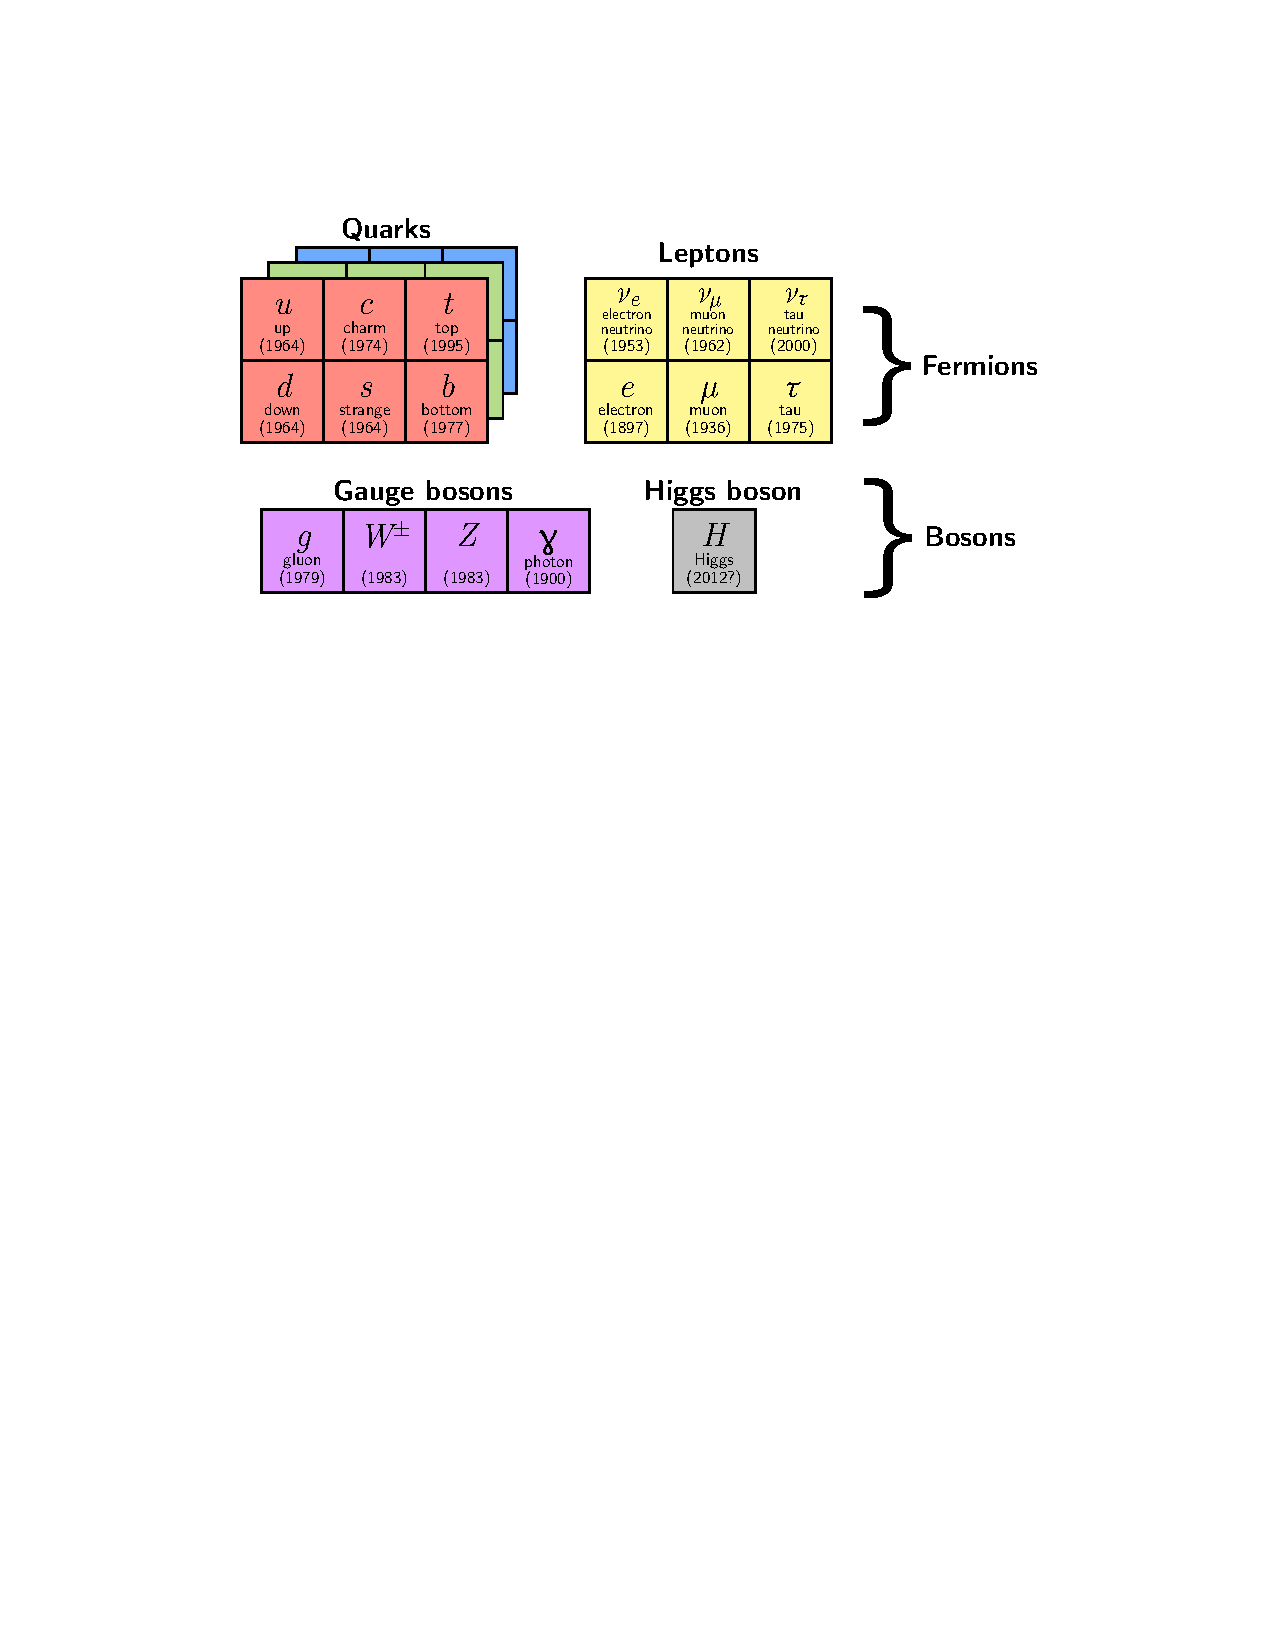
\includegraphics[width=0.95\textwidth]{figures/standardmodel/particles_reece}
  \caption{Simplified illustration of the fundamental particles of the Standard Model~\cite{2013.thesis.ryan}, where the parenthetical note to each particles indicates the year of discovery.}
  \label{fig:sm-particles-1}
\end{figure}

\begin{figure}[tp]
  \centering
  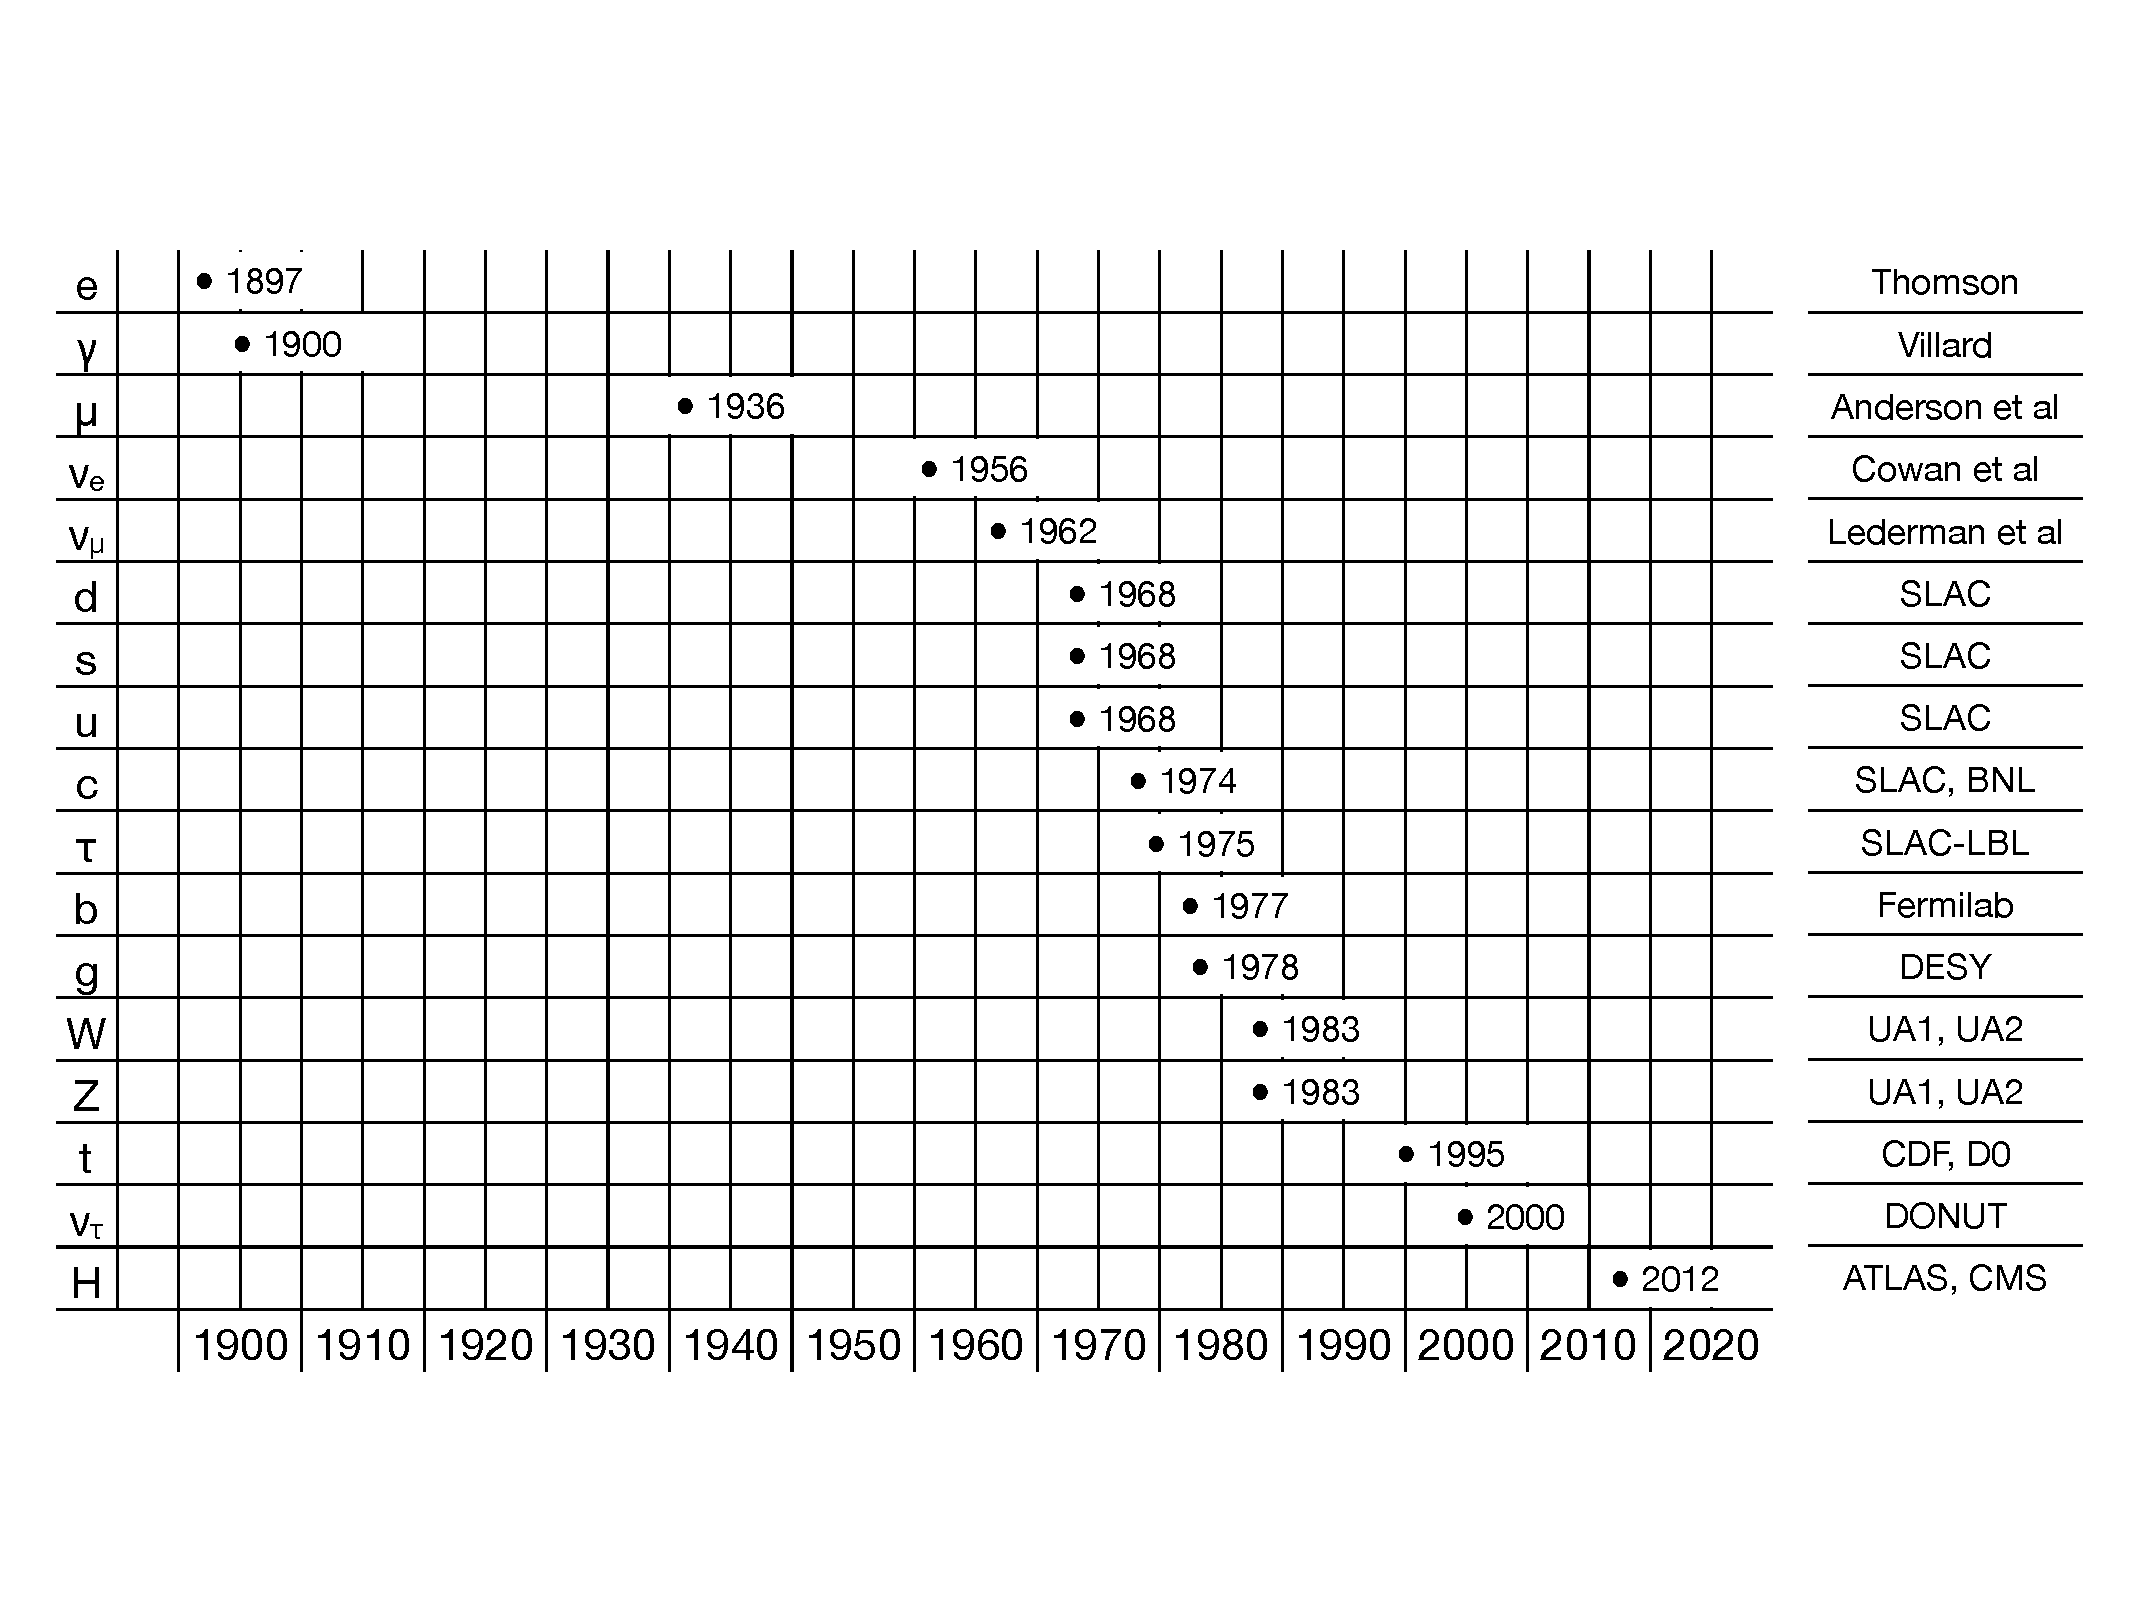
\includegraphics[width=0.95\textwidth]{figures/standardmodel/discoveries}
  \caption{Graph of the discoveries of the fundamental particles of the Standard Model versus time.}
  \label{fig:sm-particles-2}
\end{figure}

\section{Search for the Higgs}

Despite the strong theoretical motivation for the existence of the Higgs boson, it was not verified for nearly fifty years after its initial proposal. The topic of experimental observation was approached by Ellis, Gaillard, and Nanopoulos, who decided ``we do not want to encourage big experimental searches for the Higgs boson''~\cite{1976.higgspheno} because its mass was an unknown parameter and its couplings to other particles ``are probably all very small''~\cite{1976.higgspheno}.

\begin{figure}[tp]
  \centering
  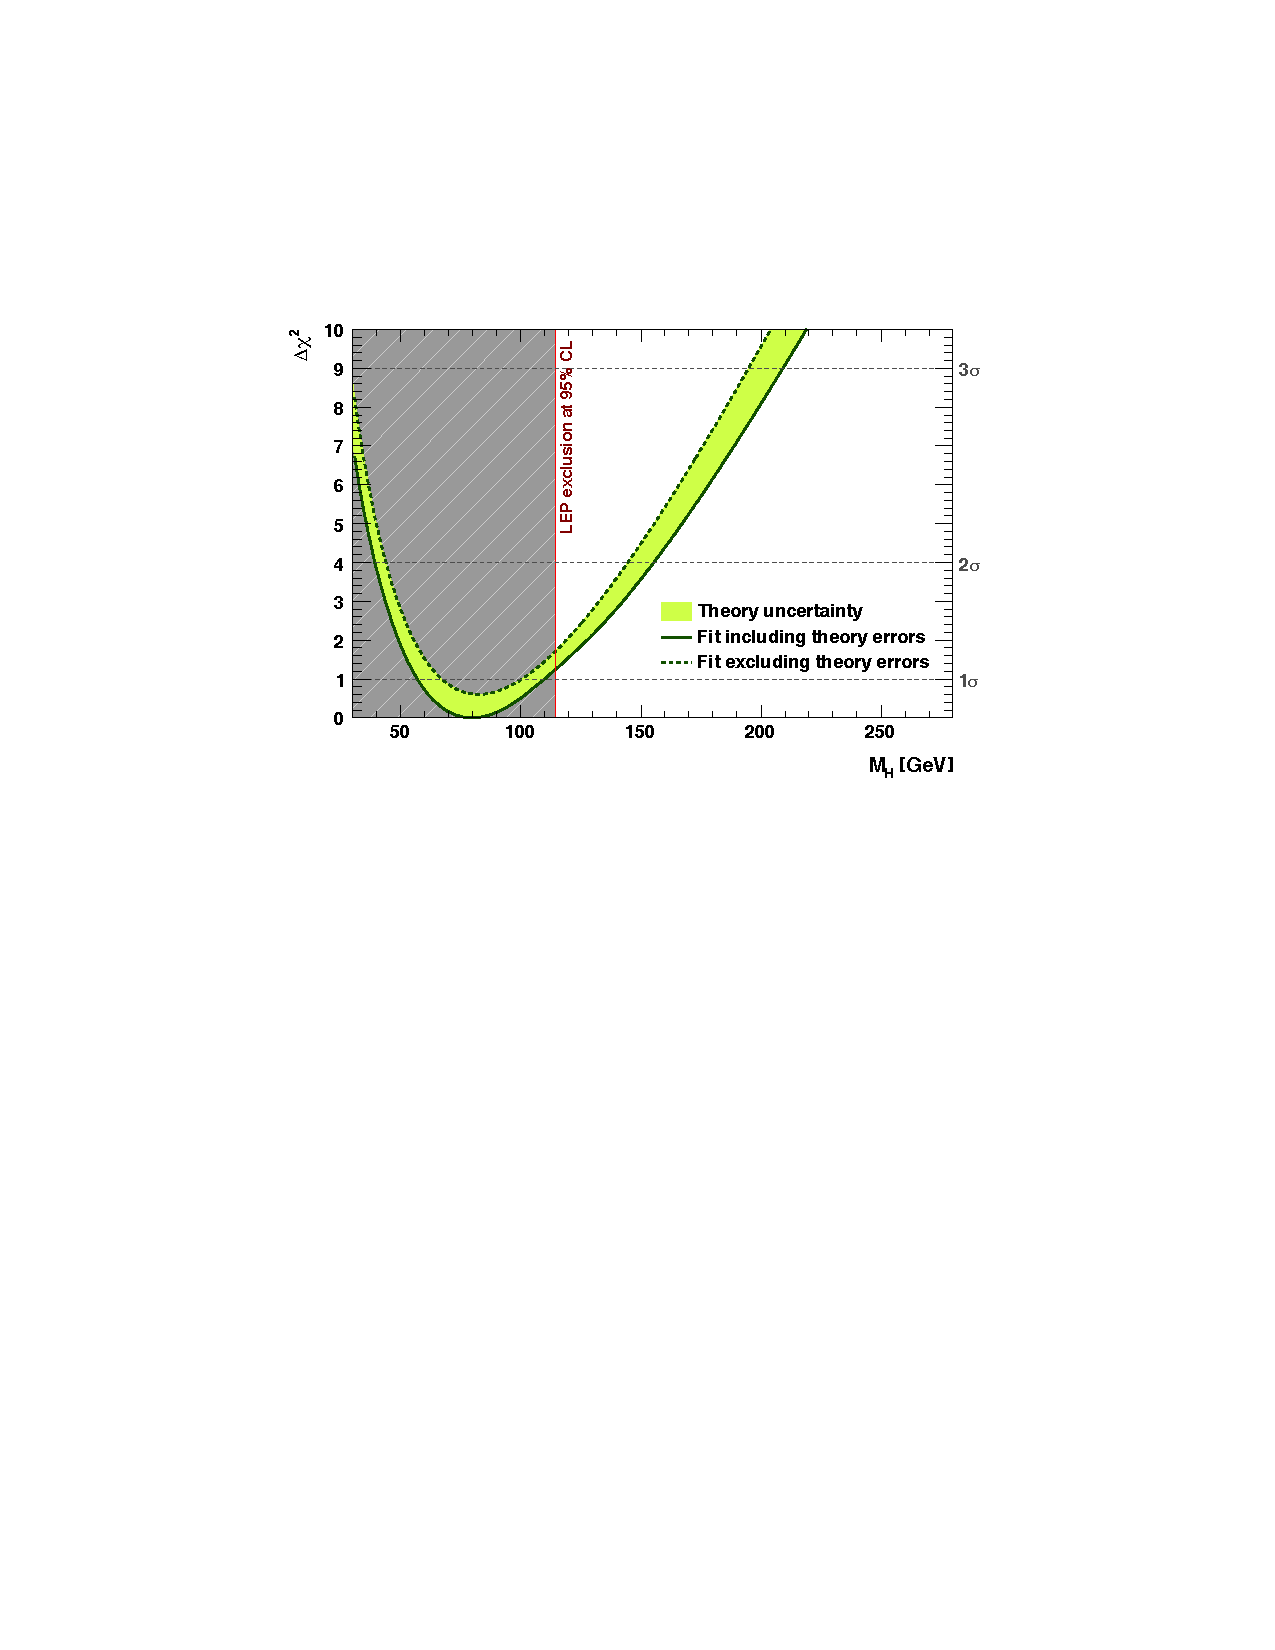
\includegraphics[width=0.48\textwidth]{figures/standardmodel/gfitter_standardfit}
  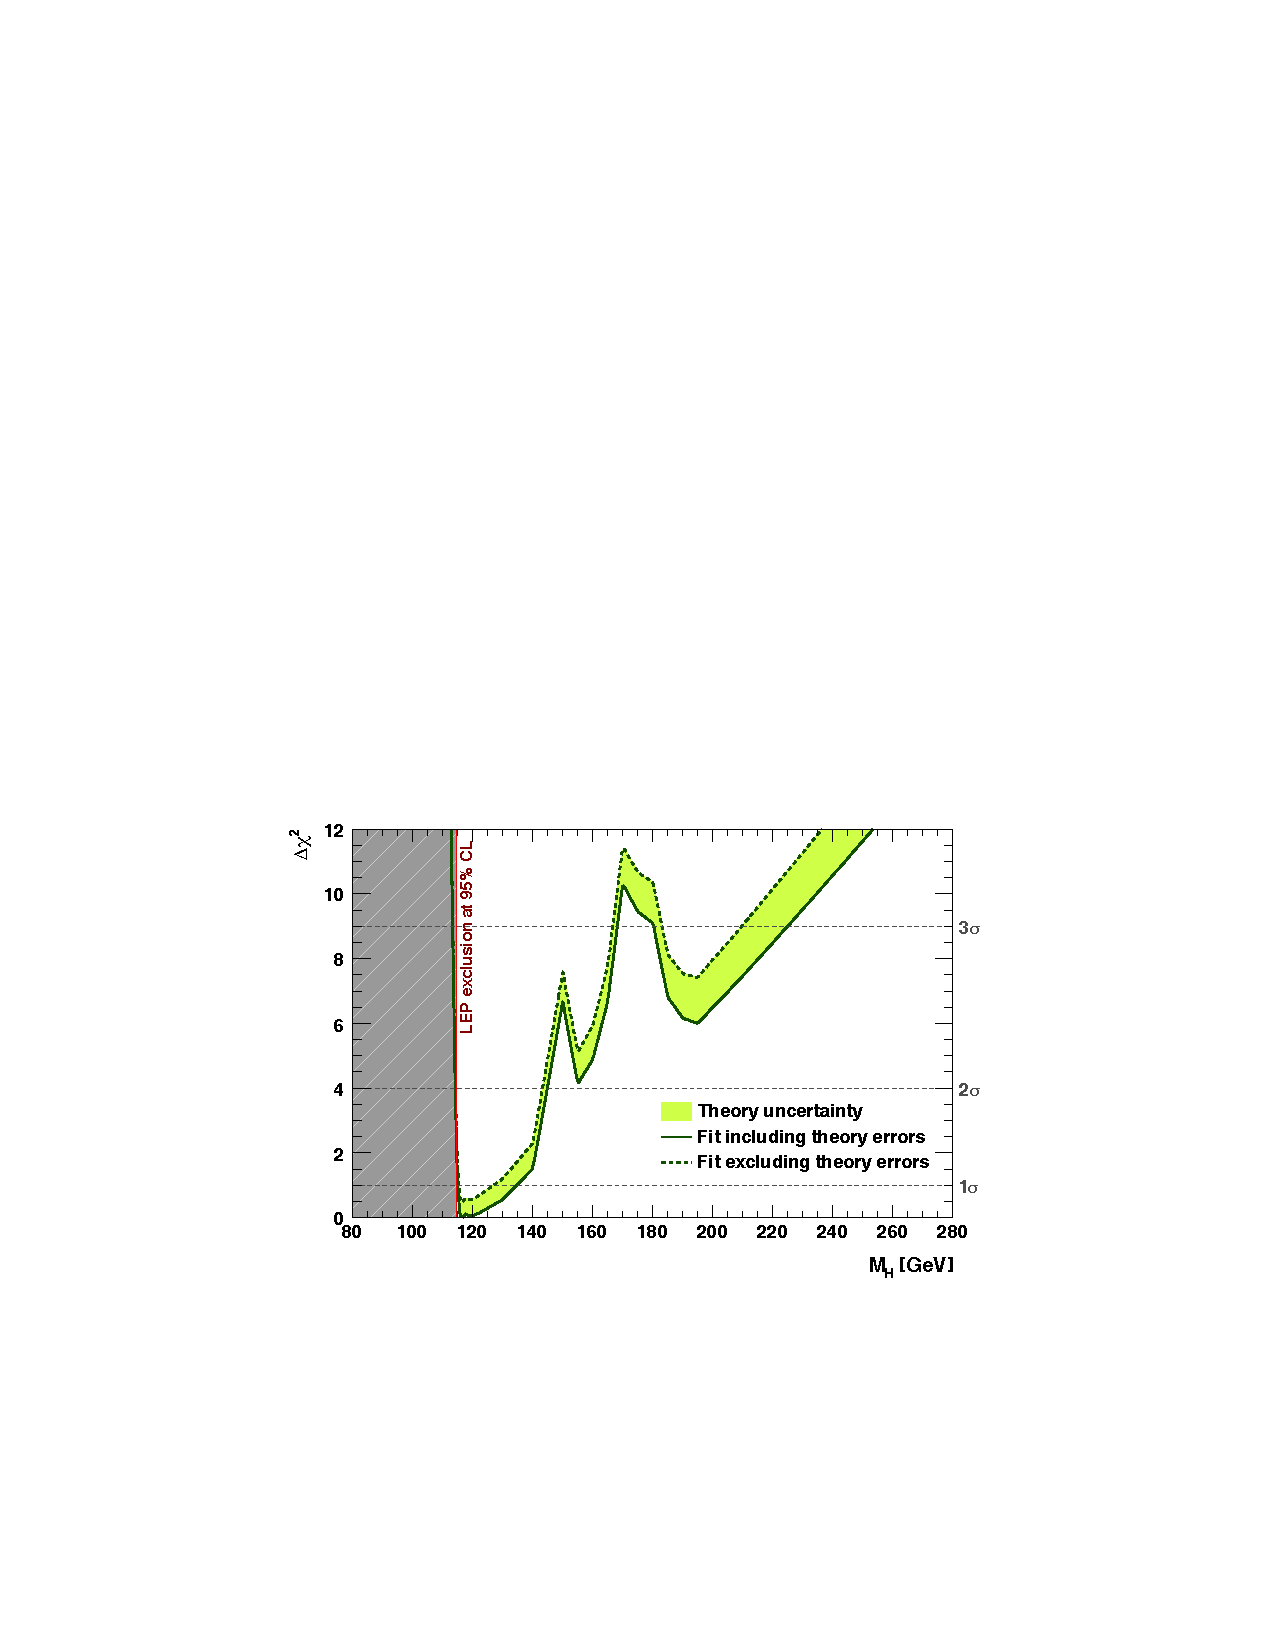
\includegraphics[width=0.48\textwidth]{figures/standardmodel/gfitter_completefit}
  \caption{Summary of the preferences for the Higgs mass as a result of global fits to precision electroweak data~\cite{2009.gfitter} without direct Higgs searches from LEP and the Tevatron (left) and with (right). The fits are done before LHC data-taking.}
  \label{fig:sm-gfitter}
\end{figure}

The largest production modes of the Higgs boson are through gluon fusion (ggF), vector boson fusion (VBF), and production in association with a vector boson ($VH$), and the cross-sections for these processes are indeed small. 

The search for the Higgs boson was among the major goals of experiments at the Large Electron-Positron Collider (LEP)~\cite{2003.lep-higgs} and the Tevatron proton-antiproton collider~\cite{2013.tevatron-higgs}.

The production mechanisms which have been most searched for are shown in \cref{fig:sm-higgs-diagrams} with their cross-section for the Higgs mass at 125 GeV.

\begin{figure}[tp]
  \centering
  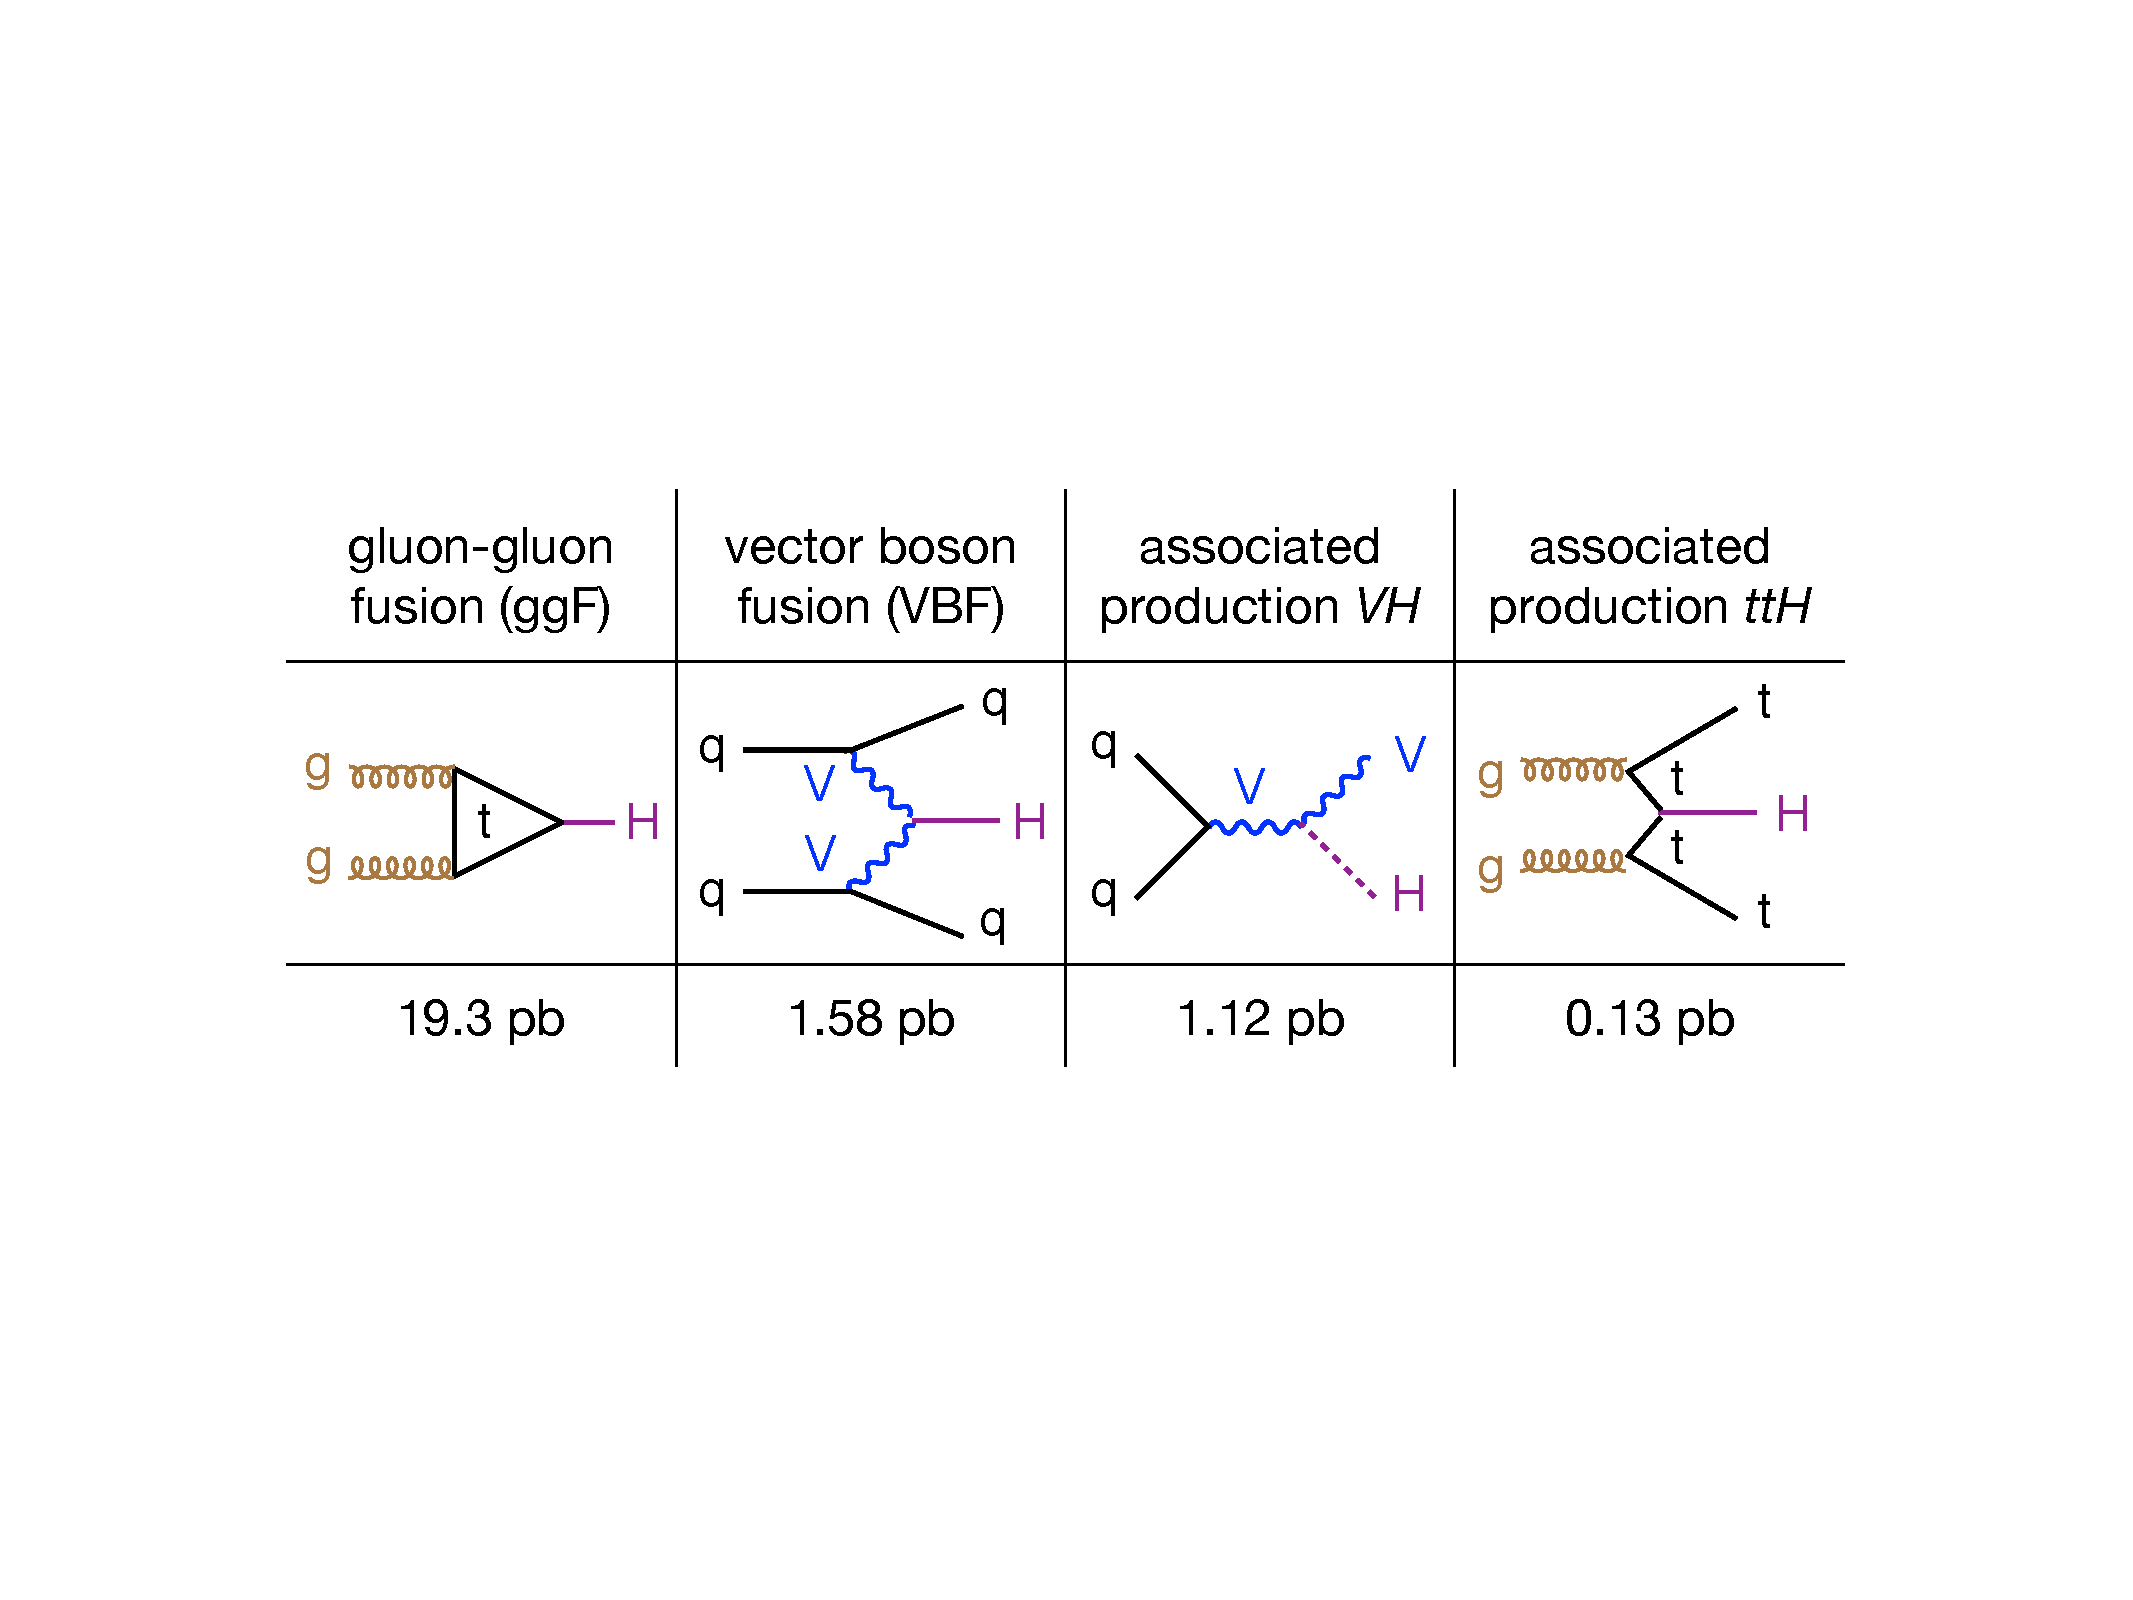
\includegraphics[width=0.95\textwidth]{figures/standardmodel/higgsproductions}
  \caption{Selected Higgs boson production mechanisms and their cross-sections for $m_H \!=\! 125$ GeV~\cite{2013.lhchxswg}.}
  \label{fig:sm-higgs-diagrams}
\end{figure}

\section{Shortcomings}

\begin{description}
    \item[Dark matter] \hfill \\
      Pass.
    \item[Gravity]     \hfill \\
      Pass.
    \item[Hierarchy]   \hfill \\
      Pass.
\end{description}

